\documentclass[a4paper]{scrreprt}
\setcounter{tocdepth}{3}
\setcounter{secnumdepth}{3}

\usepackage[german]{babel}
\usepackage[utf8]{inputenc}
\usepackage[T1]{fontenc}
\usepackage{ae}
\usepackage{graphicx}
\usepackage{lscape} % querformat
\usepackage{tabu}
\usepackage{hyperref}
\usepackage{xcolor}
\usepackage[toc]{glossaries}
\usepackage{pgfplots}
\usepackage{float}
\makeglossaries

\newglossaryentry{Unittest}
{
  name=Unittest,
  description={Auch bekannt als Modul- oder Komponententest. Wird in der Softwareentwicklung angewendet, um die funktionalen Einzelteile (Units) von Computerprogrammen zu testen, d. h., sie auf korrekte Funktionalität zu prüfen}
}

\newglossaryentry{Hallway Usability Test}
{
  name=Hallway Usability Test,
  description={Test, bei dem zufällige Personen zum Testen von Softwareprodukten und -schnittstellen verwendet werden}
}

\newglossaryentry{Qualitaetssicherung}
{
  name=Qualitätssicherung,
  description={Letzte Phase des Wasserfallmodells}
}


\begin{document}
\title{Testbericht}
\author{Fangzhou Bian, Kathrin Blum, Matthias Bruns, \\Leonhard Duda, Tan Grumser, Yuguang Lin}
\maketitle
%\Footnote für Fußnoten
% Platzierung des Inhaltsverzeichnisses
\tableofcontents



\chapter{Einleitung}

Dieses Dokument verschafft einen Überblick über die \Gls{Qualitaetssicherung} des Projekts. In dieser Phase wurde die Überdeckung der \Gls{Unittest}s maximiert, die Testszenarien des Pflichtenhefts durchgegangen und gefundene Fehler behoben. Des Weiteren wurde ein \Gls{Hallway Usability Test} durchgeführt. Die dokumentierten Tests wurden wieder unterteilt in einen Server- und Clientteil.

\chapter{Server}

\section{Bug Fixes}

\begin{itemize}
\item Sceduler\\ \\
Symptom: Die Funktionen die einmal täglich aufgerufen werden sollten, wurden nicht ausgeführt. TimeController.deleteGroups() und TimeController.updateMensaData() wurden nicht aufgerufen.\\ \\
Ursache: Die Annotationen @Component hat in der Klasse TimeController hat gefehlt, damit hat SpringBoot die Klasse nicht gefunden und den Sceduler nicht Initialisiert.\\ \\
Behebung:  Die Annotation wurde hinzugefügt.
\end{itemize}


\section{Unittests}
Für die Unit Tests wurde das Framework JUnit verwendet. Die Testabdeckung am Server wurde mit EclEmma überprüft.

\begin{itemize}

\item GroupController - Test
getestete Funktionalitäten, zusätzlich zu den bisherigen aus letztem Dokument
\begin{itemize}


\item getGroupByPreferecne
Test: Zwei Testgruppen wurden dem Repository hinzugefügt jeweils mit der selben meetingTime, aber unterschiedlichen Essenslinien
Dann wurde die Methode getGroupByPreference mit Start und Endzeit, sodass beide Gruppen sie erfüllen und einem Array aus Essenslinien, von denen es nur eine Übereinstimmung mit den Gruppen gibt, aufgerufen.
Da GetGroupByPreference sowohl die angegebenen Zeiten, als auch die Essenslinien berücksichtigt, dürfte nur eine Gruppe zurückgegeben werden.
zum überprüfen würde die Länge des zurückgegebenen Arrays überprüft.
\\ \\
Test2: Analog zu oben, nur dass keine Gruppe eine übereinstimmende Essenslinie mit den Preferenzen hatte.
Ziel war es zu sehen, ob ein Array der Länge 0 zurückgegeben wird oder unerwartetes Verhalten auftritt.
Wie erwartet hatte das zurückgegebene Array die Länge null.
\\ \\
Test3: Analog zu oben, gruppen haben passende Essenslinie aber nur eine Gruppe hat eine passende (Rand) Uhrzeit, und wie erwartet wird genau diese Gruppe zurückgegeben.
\end{itemize}

\item UserController - Test 
getestete Funkitonalitäten zusätzlich zu denen aus letztem Dokument

\begin{itemize}

\item DeleteUser
Test 1: Ein User ("User1") wurde anhand seines Tokens ins Repository hinzugefügt. Nun wird versucht einen anderen User ("User2"), der nicht im Repository liegt, aus dem Repository zu löschen. Wie erwartet, wird dabei kein anderer User gelöscht, sondern eine ResponseStatusException geworfen.

\item DeleteAllUser
Test1: Zwei User werden ins Repository hinzugefügt. Danach wird DeleteAllUser aufgerufen, nun sollte kein User mehr im Repository liegen. Beim Versuch auf einen der User mit der Methode "User getUser(String token)" aus dem Repository zu holen, wird eine ResponseStatusException geworfen. 

\item IntitalizeAdminUser
Test 1: Die Methode intializeAdminUser wird aufgerufen, da es noch keinen AdminUser gibt, wird einer neu angelegt. Um das zu überprüfen, prüfen wir, dass das angelegte Userobjekt nicht leer ist.

Test 2: Die Methode initalizeAdminUser wird zweimal aufgerufen. Beim ersten Aufruf wird ein Admin User angelegt, beim zweiten Aufruf sollte nichts passieren, da bereits ein Admin User existiert. 
\end{itemize}
\end{itemize}

\section{Testszenarien}

Die nachfolgenden Tests laufen ausschließlich auf dem Server und sind dazu da die klassenübergreifende Funktionalitäten zu testen.\\


\begin{itemize}

\item Szenario 1 (MK60, MK 80, MK100)\\
Vorbedingung: Es ist bereits User Alice im UserRepository. Dieser User ist in keiner Gruppe.\\
Ablauf: Der User erstellt eine Gruppe und verlässt sie anschließend wieder.\\
Nachbedingung: Der User ist in keiner Gruppe und die erstellte Gruppe hat sich gelöscht, als Alice, als letzter User ausgetreten ist.\\


\item Szenario 2 (MK70, MK 80)\\
Vorbedingung: Es existieren die User A,B und C. Es existiert eine Gruppe X die mit User A und B voll ist. \\
Ablauf: User B verlässt die Gruppe, sodass Platz für User C frei wird. Dieser tritt dann der Gruppe bei.\\
Nachbedingung: User A und C sind in Gruppe X und User B ist in keiner Gruppe.\\


\item Szenario 3 (MK 100)\\
Vorbedingung: Es existiert ein User A der in der Gruppe X ist.\\
Ablauf: Es werden (um Mitternacht) alle Gruppen gelöscht.\\
Nachbedingung: User A  ist in keiner Gruppe und die Gruppe X existiert nicht mehr.\\

\item Szenario 4 (MK110)\\
Vorbedingung: Es existiert ein User A der in der Gruppe X ist und ein Admin User.\\
Ablauf: Die Gruppe X wird von dem Admin User gelöscht.\\
Nachbedingung: User A  ist in keiner Gruppe und die Gruppe X existiert nicht mehr.\\


\end{itemize}

\chapter{Client}

\section{Allgemeines zum Testen und Verbessern}

Die meisten Fehler wurden bereits beim „Ausprobieren“ der App bemerkt und mit dem Debugger lokalisiert, sodass passende Verbesserungen durchgeführt werden konnten. Durch Unit- und Integration-Tests wurden kaum noch Fehler gefunden, dafür aber Funktionalität der Verbesserungen abgesichert. Im Folgenden sind daher die Funktionalitäten der wichtigsten Klassen nach den Verbesserungen und dazu jeweils die diese absichernden Tests aufgelistet. Anschließend werden die Ergänzungen und Veränderungen seit der letzten Phase aufgezeigt und die Motivation dahinter, soweit nicht noch beschrieben, erklärt.
Für die Unit-Tests reichte die in Android-Studio standardmäßig installierte Software nicht aus. Grund dafür ist, dass diese Testsoftware zu viele verwendete komplexere Klassen stubt und mockt, um die Tests schneller und unabhängiger zu machen. Eine Klasse wie Pair<String, State>, die essentiell für die Kommunikation zwischen ViewModel und Activity ist, wird bei den Tests durch einen leeren Stub ersetzt, der das Testen unmöglich macht. Daher mussten weitere Frameworks benutzt werden.

\section{Tools zum Testen}

\subsection{Robolectric}
Robolectric ist ein Framework für Tests in Android Studio, das in Sachen Stubbing und Mocking von verwendeten Klassen geschickter vorgeht als der Standard in Android Studio. Klassen wie Pair werden nicht gestubt, sodass deren Funktionalität gewährleistet ist und sinnvolles Testen möglich wird. Daher wurde dieses Framework installiert.

\subsection{Mockito und Powermockito}
Bei Unit-Tests ist die Überschaubarkeit des Testbereichs wichtig, daher müssen Klassen und Funktionen, die zu weit aus dem Testbereich hinausführen, gemockt werden, wozu sich Mockito eignet. Was Mockito jedoch nicht kann, ist unter anderem, statische Klassen und Methoden zu mocken. Diese werden in MensaMeet bei Serveranfragen verwendet. Abhilfe schafft hier die Erweiterung Powermockito.

\subsection{Espresso}
Mit Espresso ist es möglich Tests in der laufenden App durchzuführen. Man ersetzt damit einen menschlichen Tester, der sich durch die App klickt und testet ob alles so funktioniert wie es soll. Der Hintergrund dabei ist, dass man die Tests automatisiert durchführen möchte und man auch in der Lage sein will, ein Testszenario zu reproduzieren, um die Fehlerursache ausfindig zu machen. Espresso macht genau diese Dinge möglich und nimmt dem Programmierer so jede Menge Arbeit beim Testen ab.

\section{Models}
\subsection{IdEnum}
Das Interface IdEnum wurde neu eingeführt, um die Umwandlung von Enums mit Konstante-String-Paaren wie Gender, Status und Subject in SpinnerItem-Objekte für die Darstellung in Spinnern (Auswahllisten) zu erleichtern. Zuvor wurde nicht mit Wertepaaren gearbeitet (siehe MensaMeetItem -> E \& V -> Handhabung von Wertepaaren mit representedValues und SpinnerItem), was problematisch war. Die obengenannten Enums und MealLines implementieren dieses Interface.

\subsection{MensaMeetSession}
Dies ist das Singleton, das alle wichtigen activityübergreifenden Daten einer Sitzung wie den aktuellen Benutzer und seine Linienauswahl speichert. \\
\textbf{Elemente (Auswahl)}

\begin{itemize}
\item Attribut user \\
Dies ist der aktuelle Benutzer. Es ist genau dann null, wenn kein Benutzer eingeloggt ist, und kann in diesem Sinne abgefragt werden. Die Gruppe, der der Benutzer beigetreten ist, wird in dessen Attribut groupToken spezifiziert.
\item Methode userDataIncomplete \\
Sie gibt an, ob die Profildaten des aktuellen Benutzers noch nicht ausreichend spezifiziert sind, also ob eine der obligatorischen Angaben Name und Status noch fehlt.
\item Attribut createdGroup \\
Hier wird der Gruppenentwurf des Benutzers nach dem Verlassen von CreateGroupActivity gespeichert, auch wenn er unvollständig ist, damit der Benutzer ihn zu einem späteren Zeitpunkt weiter bearbeiten kann.
\item Methode createdGroupDataIncomplete \\
Sie überprüft, ob die Angaben des Gruppenentwurfs vollständig sind, sodass sie zum Server geschickt werden kann.
\item Methode initialize \\
Mit ihr werden die Daten in MensaMeetSession zu Beginn einer Sitzung initialisiert. Die meisten Daten werden auf null gesetzt, der Parameter user als user gesetzt, der Speiseplan vom Server geladen.
\item Methode invalidate \\
Das Gegenstück zu initialize, dass am Ende einer Sitzung alle Daten auf null setzt.
\end{itemize}

\textbf{Ergänzungen und Verbesserungen seit der letzten Phase}

\begin{itemize}
\item Verzicht auf Attribut chosenGroup \\
Die vom Benutzer ausgewählte Gruppe wird nur noch als groupToken in seiner Klasse spezifiziert. Es ist nicht sinnvoll, das ganze Group-Objekt zu speichern, da es sich ständig durch neue Mitglieder oder durch Löschung verändern kann. 
\item Verzicht auf Attribut receivedGroup \\
Zuvor wurden die passenden Gruppen, die bei SelectGroupActivity vom Server geladen werden, in der Session-Datei gespeichert. Dies ist jedoch nicht nötig, da sie außer in SelectGroupActivity nirgends mehr gebraucht werden.
\item createdGroupDataIncomplete hinzugefügt
\item initialize und invalidate hinzugefügt \\
Dadurch werden Ein- und Ausloggen standardisiert.
\item Prinzip “Kein aktuelles User-Objekt, keine Sitzung“ \\
Scheitert das Anfordern des User-Objekts für den aktuellen Benutzer vom Server, so wird die Sitzung sofort beendet. Zum einen kann es immer sein, dass der aktuelle Benutzer zwischenzeitlich gelöscht wurde, zum anderen ist sind ohne aktuelles User-Objekt keine sinnvollen Aktionen in der App mehr möglich. Der Benutzer müsste versuchen, sich neu einzuloggen.

\end{itemize}

\section{Util-Klassen}

\subsection{HTTPUtil}
Die Klasse HTTPUtil dient zur Kommunikation mit dem Server. Ihre Methoden entsprechen größtenteils bekannten Standard-Beispielen. \\
\textbf{Ergänzungen und Verbesserungen seit der letzten Phase} \\
\begin{itemize}
\item Weiterleitung der Serverantwort auch bei Fehler \\
Die bisherige Implementation der Methode fetch lieferte nur die Serverantwort als JSON-String, wenn kein Fehler vorlag. Ansonsten wurde eine Exception geworfen und die Methode ohne lesen der Serverantwort beendet. Es war jedoch wünschenswert, den genauen Fehlercode und die Fehlermeldung in der App auswerten und gegebenenfalls an den Benutzer weiterleiten zu können. Daher würde die Methode dahingehend verändert, dass sie im Fehlerfall keine Exception, dafür aber den JSON-String der Serverantwort, der Fehlercode und -meldung weitergibt.
\end{itemize}

\subsection{RequestUtil}
Die Methoden der Klasse RequestUtil entsprechend den Diensten, die der MensaMeet-Server anbietet. Sie akzeptieren Objekte der Klassen, die verarbeitet werden sollen, serialisieren sie zu JSON und führen mit Hilfe von HTTPUtil die konkreten Serveranfragen durch. Die JSON-Antwort wird dann wieder zu den jeweiligen Objekten deserialisiert und an den Aufrufer der Methode zurückgegeben. \\

\textbf{Elemente} \\

\begin{itemize}
\item Methode createUser
\item \textit{util.RequestUtilTest.userTest()}
\item Methode getUser
\item \textit{util.RequestUtilTest.userTest()}
\item Methode updateUser
\item \textit{util.RequestUtilTest.userTest()}
\item Methode deleteUser
\item \textit{util.RequestUtilTest.tearDown()}
\item Methode createGroup
\item \textit{util.RequestUtilTest.groupTest()}
\item Methode getGroup
\item \textit{util.RequestUtilTest.groupTest()}
\item Methode getGroupByPrefferences
\item \textit{util.RequestUtilTest.groupTest()}
\item Methode deleteGroup
\item \textit{util.RequestUtilTest.groupTest()}
\item Methode addUserToGroup
\item \textit{util.RequestUtilTest.groupTest()}
\item Methode removeUserFromGroup
\item \textit{util.RequestUtilTest.groupTest()}
\item Methode getMensaData
\item \textit{util.RequestUtilTest.mensaDataTest()}
\item Klasse GroupForRequest \\
\textit{Diese Klasse ist nötig, da sich die Group-Klasse, die vom Server verlangt wird, von der im Client unterscheidet. Im Client sind die Zeiten zur als Date-Objekte, beim Server als Strings hinterlegt. Der Konstruktor und die Methode parseToGroup dienen zur Umwandlung.}
\item Klasse GroupForRequestWithToken \\
\textit{Diese Klasse ist nötig, da beim Erstellen einer neuen Klasse ein Group-Objekt ohne das Attribut token an den Server übertragen muss, um von diesem ein Group-Objekt mit servergeneriertem Token zu erhalten. Diese Klasse enthält token, die Klasse GroupForRequest nicht.   }
\item Klasse GroupWithPrefferences \\
\textit{Diese Klasse entspricht dem JSON-Objekt, das bei einer Anfrage in getGroupByPrefferences dem Server übermittelt wird.}
\item Klasse RequestException
\textit{Diese Exception dient dazu, den Aufrufer einer Methode von RequestUtil bei einem vom Server verursachten oder sonstigen Fehler zu benachrichtigen und ihm Informationen zum Fehler zu übergeben. Ein Konstruktor liest aus dem aus der Serverantwort erzeugten JsonNode Fehlercode- und Fehlernachricht und speichert sie. Liegt kein Serverfehler vor, werden die Daten von eventuell auftretenden anderen Exceptions weitergeleitet. } \\

\textbf{Ergänzungen und Verbesserungen seit der letzten Phase}

\item GroupForRequestWithToken \\
\textit{Zuvor wurden keine servergenerieten tokens vom Server empfangen, da immer ein Group-Objekt mit Attribut token gesendet und dieses vom Server übernommen wurde. Ein servergeneriertes Token ist jedoch notwendig für die eindeutige Identifizierbarkeit einer erstellten Gruppe. }
\item Weiterleitung von Server- und anderen Exceptions \\
\textit{Zuvor konnte man einen Fehler nur erkennen, wenn das von einer Methode in RequestUtil zurückgegebene Objekt nicht den Erwartungen entsprach. Dies war jedoch nicht eindeutig und aussagekräftig.}

\end{itemize}

\section{Activity-ViewModel-, List-ListHandler und Item-ItemHandler Paare}

Die Activities sowie ihre Unterelemente Lists und Items sind für die Darstellung der Benutzeroberfläche zuständig, während die zugehörigen ViewModels und Handlers die Logik dahinter enthalten. \\

Die Activity-Viewmodel-Paare sind nach ihrem frühestmöglichen Erscheinen in einem Benutzungsdurchlauf geordnet. Die Beschreibung des Verhaltens geschieht in chronologischer Reihenfolge. \\

\subsection{MensaMeetActivity und MensaMeetViewModel} 
MensaMeetActivity ist die abstrakte Oberklasse aller Activities in MensaMeet, MensaMeetViewModel die abstrakte Oberklasse aller ViewModels. Beide Klassen enthalten Attribute, Methoden und Vorgänge, die in mehreren oder allen Activities und ViewModels benötigt werden. \\
 \subsubsection{Elemente in MensaMeetActivity} 
 
 \begin{itemize}
 \item Methode onCreate \\
 \textit{Sie ruft onCreate der Oberklasse AppCompatActivity auf und sollte immer am Anfang der onCreate-Methode einer Unterklasse aufgerufen werden, da die Activity sonst teilweise nicht richtig dargestellt wird. Zudem enthält sie die Anweisung, dass die App immer vertikal angezeigt wird und nicht gedreht wird, da dabei unerwünschtes Verhalten auftreten kann, dessen Behandlung zusätzlichen Aufwand erfordert.}
\item Attribut viewModel \\
\textit{Das zur Activity gehörende ViewModel}
\item Methode initializeViewModel \\
\textit{Jede Unterklasse der Activity kann diese Methode an beliebiger Stelle benutzen, um dem Attribut viewModel das konkrete ViewModel zuzuweisen. Die Initialisierung des Attributs ist Vorbedingung für den Aufruf weiterer Methoden, die darauf zugreifen.}
\item Methode checkAccess\\
\textit{Sie überprüft, ob die Zugangsbedingungen zur Activity erfüllt sind. Da sie leer ist und auch nicht standardmäßig in einer anderen Methode aufgerufen wird, ist sie eher als Anregung für die Unterklassen zu verstehen. In diesen Enthält sie neben einer Auswertung den Befehl, die Activity im negativen Fall zu beenden, wobei der Benutzer in die vorhergehende Activity im Activity-Stack zurückfällt. Da sie meistens über das ViewModel auf MensaMeetSession zugreift, muss sie nach der Methode initalizeViewModel aufgerufen werden.}
\item Methode observeLiveData\\
\textit{Sie beobachtet das SingleLiveData-Objekt eventLiveData des ViewModels und muss daher nach initializeViewModel aufgerufen werden. Das Objekt dient zur Kommunikation des ViewModels mit der Activity, das nach dem MVVM-Modell nicht direkt auf die Activity zugreifen darf. Falls das ViewModel eventLiveData ändert, wird die Activity benachrichtigt und kann den veränderten Wert auslesen, der eine Statusänderung und eine zugehörige Nachricht enthält. Zur Auswertung dieser Veränderung wird die Schablonenmethode processStateChange aufgerufen.}
\item Methode processStateChange\\
\textit{Sie wird bei Veränderung von eventLiveData im ViewModel aufgerufen und wertet die Änderung aus, die einen neuen Status und eine zugehörige Nachricht enthält. Jede Activity kann sie individuell überschreiben.}
\item Methode showMessage\\
\textit{Sie blendet eine Kombination aus einer gegebenen Stringressource und der über eventLiveData vom ViewModel übermittelten Nachricht, die zum Beispiel vom Server stammt, in Form eines Toasts (temporär angezeigtes Nachrichtenfeld am unteren Bildschirmrand) ein. Damit lassen sich zum Beispiel Serverfehler anzeigen.}
\item Attribute buttonHome, buttonNext und buttonBack\\
\textit{Diese Buttons werden in den meisten Activities angezeigt.}
\item Methode initializeButtons\\
\textit{Sie findet mit Hilfe der View-Ids die Buttons in der View der Activity und weist sie den entsprechenden Attributen zu. Daher sollte die Methode erst dann aufgerufen werden, wenn die View der Activity initialisiert wurde. Zudem weist sie den Buttons ClickListener zu, die auf die Methoden onClickHome, onClickNext und onClickBack verweisen.}
\item Methoden onClickHome, onClickNext und onClickBack\\
\textit{Sie werden beim Klicken auf die jeweiligen Buttons aufgerufen und können von den Unterklassen überschrieben werden, um das Verhalten anzupassen}
\item Methode onResume\\
\textit{Sie wird bei einer Rückkehr zur Activity aufgerufen, falls diese zwischenzeitlich in den Hintergrund getreteten ist. Selbst ruft sie wiederum onResume der Oberklasse AppCompatActivity auf und danach die Schablonenmethode reloadData}
\item Methode reloadData\\
\textit{Sie wird vom System bei der Rückkehr zur Activity aufgerufen, falls diese zwischenzeitlich in den Hintergrund getreteten ist, kann jedoch überall, auch in onCreate aufgerufen werden, falls das initiale Laden der von der Activity benötigten Daten dem erneuten Laden nach einer Rückkehr entspricht. Sie kann quasi als Auslagerungsmethode der Datenladung benutzt werden.}
\item Methoden gotoActivity und gotoHome\\
\textit{Starten eine andere Activity und leiten den Benutzer an sie weiter.}
\item Methode onBackPressed\\
\textit{Sie wird vom System bei Betätigung des Android-Back-Buttons aufgerufen und leitet zur Activity weiter, die die aktuelle Activity gestartet hat. Dies ist manchmal jedoch nicht erwünscht, die Navigation in der App soll ausschließlich über die eigenen Buttons erfolgen. Daher wird die Methode leer überschrieben und der Button generell deaktiviert.}
\item Methode goBack\\
\textit{Sie ruft onBackPressed in der Oberklasse auf und stellt somit deren Funktion zur Verfügung, falls sie doch einmal benötigt wird (siehe ShowUserActivity).}
\end{itemize}

\subsubsection{Elemente in MensaMeetViewModel}
\begin{itemize}
\item Attribut singleLiveData\\
\textit{Das SingleLiveData-Objekt, das von der Activity beobachtet wird (siehe oben).}
\item Weiteren Methoden der Klasse \\
\textit{Sie rufen jeweils entsprechende Methoden in MensaMeetSession auf. Grund dafür ist, dass nach dem MVVM-Modell die Activity nicht direkt mit dem Model kommunizieren, sondern ihre Daten vom ViewModel beziehen sollte.}
\end{itemize}

\subsubsection{Ergänzungen und Verbesserungen seit der letzten Phase}
\begin{itemize}
\item initializeViewModel, um die Zuweisung des ViewModel zu regulieren\\
\textit{Zuvor wurde das ViewModel direkt super.viewModel zugewiesen.}
\item checkAccess, um mehr ungültige Zustände zu vermeiden
\item SingleLiveEvent eventLiveData von Pair<MensaMeetViewModel, StateInterface> in Pair <String, StateInterface> geändert\\
\textit{Die vorherige Lösung stammt aus der Android-Schulung, damit das sendende ViewModel immer als Quelle mitgeliefert wird. In den Anwendungsfällen von MensaMeet ist das ViewModel jedoch immer bekannt und braucht nicht mitgeliefert zu werden. Stattdessen ist es sinnvoller, eine eventuelle Fehlernachricht als String mitzuliefern.}
\item observeLiveData, um die Beobachtung von eventLiveData im ViewModel an beliebiger Stelle initialisieren zu können\\
\textit{Zuvor war ihr Inhalt Teil der Methode onCreate, wodurch diese als super.onCreate erst nach Initialisierung des ViewModel aufgerufen werden konnte. Sie sollte jedoch immer als erstes in onCreate der Unterklassen aufgerufen werden, da es sonst zu Darstellungsproblemen wie dem Fehlen eines Hintergrundbildes kommen kann}
\item processStateChange nun in jeder Activity einheitlich genutzt\\
\textit{Zuvor gab es bei manchen Activities individuelle Lösungen.}
\item initializeButtons\\
\textit{Ihr Inhalt war zuvor ebenfalls Teil der Methode onCreate. Wenn diese jedoch als erstes in onCreate der Unterklassen aufgerufen werden soll, käme die Initialisierung der Buttons vor der Initialisierung der View der Activity, was unmöglich ist, daher die Auslagerung in eine eigene Methode.}
\item showMessage\\
\textit{Sie bündelt die oft benutzte Anweisungsfolge.}
\item Deaktivierung des Android-Back-Buttons durch leere Methode onBackPressed
\item MVVM-konformer Zugriff auf MensaMeetSession nur noch über ViewModel
\item Attribut displayMode bei ViewModel entfernt\\
\textit{Ursprünglich wurde angenommen, dass der displayMode auch für die Logik im ViewModel entscheidend sein könnte. Dies hat sich jedoch nicht bestätigt, weshalb das unnötige Attribut entfernt wurde.}
\item Methodenbeendigung nach jeder eventLiveData-Änderung \\
\textit{Zuvor wurde fälschlicherweise angenommen, dass die Methode und alle weiteren Methoden sofort beendet wurde, sobald der Beobachter benachrichtigt wird. Dies ist jedoch nicht der Fall, daher müssen die Methoden explizit beendet werden.}
\end{itemize}

\subsection{BeginActivity und BeginViewModel}
BeginActivity ist die erste Activity, die dem Benutzer nach dem Starten der App angezeigt wird. BeginViewModel enthält die Methoden, die beim Klicken der Buttons aufgerufen werden und wiederum bei der Activity den Seitenwechsel triggern (siehe MensaMeetActivity -> Elemente in MensaMeetActivity -> observeLiveData). \\

\subsubsection{Sichtbare Elemente} 
\begin{itemize}
\item Login (Button)
\item Registrieren (Button) \\
\end{itemize}

\subsubsection{Verhalten} 
\begin{itemize}
\item Die Activity ist nicht zugreifbar, wenn der Benutzer eingeloggt ist. 
\item Bei Klick auf Login kommt man zu LoginActivity \\
viewmodel.BeginViewModelTest.toLoginSuccess()
\item Bei Klick auf Registrieren kommt man zu RegisterActivity. \\
viewmodel.BeginViewModelTest.toRegisterSuccess()
\end{itemize}

\subsubsection{Ergänzungen und Verbesserungen seit der letzten Phase} 
\begin{itemize}
\item Zugriffskontrolle (siehe MensaMeetActivity -> E\&V -> checkAccess)
\end{itemize}

\subsection{LoginActivity und LoginViewModel}

Auf LoginActivity kann sich der Benutzer mit seinen Firebase-Login-Daten bei MensaMeet einloggen. LoginViewModel kommuniziert dabei mit dem Firebase-Projekt von MensaMeet und dem Server.

\subsubsection{Sichtbare Elemente}
\begin{itemize}
\item E-Mail-Adresse (Textfeld)
\item Passwort (Textfeld)
\item Login (Button)
\item Zurück (Button)
\end{itemize}

\subsubsection{Verhalten}
\begin{itemize}
\item Die Activity ist nicht zugreifbar, wenn der Benutzer eingeloggt ist.
\item Bei Klick auf Zurück gelangt der Benutzer auf BeginActivity.
\item Bei Klick auf Login wird der Login-Prozess beim ViewModel gestartet.
\item Falls ein Textfeld leer ist, Fehlermeldung.
\item Mit den Daten wird bei Firebase das Einloggen versucht. 
\item Bei erfolgreichem Einloggen wird ein User-Token empfangen. Mit diesem wird beim Server das entsprechende User-Objekt angefordert.
\item Bei gescheitertem Einloggen wird die Fehlermeldung von Firebase angezeigt.
\item Wird ein User-Objekt vom Server empfangen, wird damit in MensaMeetSession die neue Sitzung initialisiert. 
\item Wird kein User-Objekt empfangen, wird der Benutzer bei Firebase wieder ausgeloggt und die Fehlermeldung des Servers angezeigt. Grundsatz: kein aktuelles User-Objekt, keine Sitzung. Der Benutzer verbleibt in der Activity.
\item Sind die Angaben im User-Objekt ausreichend (Name und Status dürfen nicht leer sein), wird der Benutzer zu HomeActivity weitergeleitet.
\item Sind die Angaben im User-Objekt nicht ausreichend, wird der Benutzer zu UserActivity weitergeleitet, damit er sie dort ergänzen kann.

\end{itemize}

\subsubsection{Ergänzungen und Verbesserungen seit der letzten Phase}
\begin{itemize}
\item Zugriffskontrolle (siehe MensaMeetActivity -> E\&V -> checkAccess)
\item Initialisierung der Sitzung bereits hier
\item Verhalten beim Scheitern der Server-Anfragen
\item Zurück-Button (siehe MensaMeetActivity -> E\&V -> Deaktivierung des Android-Zurück-Buttons)
\item Richtiger Umgang mit leeren Eingabefeldern\\
\textit{Zuvor stürzte die App immer ab. Grund war, dass leere Eingabefelder nicht erkannt wurden, da sie immer standardmäßig einen Leerstring enthalten und nicht wie erwartet null. Der Leerstring wurde an Firebase übermittelt, wodurch es zu einer Exception und dem Absturz der App kam. Dies wurde behoben, indem auch der Leerstring erkannt wird.}
\item Methode matchPattern zur Datenüberprüfung im ViewModel entfernt\\
\textit{In der danach aufgerufenen Methode login findet auch eine Überprüfung statt.}
\item Fehlermeldung von Firebase nun an Benutzer übermittelt

\end{itemize}

\subsection{UserActivity und UserViewModel}
Auf UserActivity kann der Benutzer die von ihm veränderbaren Daten seines MensaMeet-Benutzerprofils bearbeiten. UserViewModel lädt und speichert die Daten beim Server. 

\subsubsection{Sichtbare Elemente}

\begin{itemize}
\item Auswahlbereich für Benutzerbild
\item Name (Textfeld)
\item Motto (Textfeld)
\item Geburtsdatum (Textfeld mit Auswahldialog)
\item Geschlecht (Auswahlliste)
\item Status (Auswahlliste)
\item Fachrichtung (Auswahlliste)
\item Verwerfen (Button), nicht immer angezeigt (siehe Verhalten)
\item Home (Button) 
\item Speichern (Button)

\end{itemize}

\subsubsection{Verhalten}

\begin{itemize}
\item Die Activity ist nur zugreifbar, wenn der Benutzer eingeloggt ist.
\item Falls die Benutzerdaten nicht ausreichend sind (Name oder Status leer), wird der Verwerfen-Button nicht angezeigt. Der Benutzer kann die Änderungen zwar immer noch über den Home-Button verwerfen, soll aber dazu animiert werden, seine Daten zu vervollständigen und zu speichern.
\item Bei (Wieder-)Eintritt in die Activity wird vom ViewModel das User-Objekt des Benutzers jedes Mal neu vom Server geladen und in MensaMeetSession gespeichert. \\
\textit{viewmodel.UserViewModelTest.reloadingUserFailed()}
\item Die Activity bindet ein UserItem im DisplayMode BIG\_EDITABLE ein, in dem alle Elemente außer der Navigationsbuttons enthalten sind.
\item Der Auswahlbereich für das Benutzerbild, ein UserPictureItem im DisplayMode BIG\_EDITABLE, zeigt das aktuelle Benutzerbild an. Falls noch keins ausgewählt wurde, wird das Default-Bild angezeigt. 
\item Bei Klick auf den Auswahlbereich für das Benutzerbild öffnet sich eine Liste von Benutzerbildern. Wird eins angeklickt, wir dieses als neues Benutzerbild ausgewählt.
\item Ist noch kein Geburtsdatum spezifiziert, wird ein Platzhaltertext angezeigt.
\item Bei Klick auf das Feld des Geburtsdatums wird ein Datum-Auswahldialog geöffnet.
\item Bei Klick auf Verwerfen gelangt der Benutzer auf HomeActivity, von wo er in diesem Fall gekommen sein muss. Es werden keine Daten gespeichert.
\item  Bei Klick auf Home gelangt der Benutzer auf HomeActivity, es werden keine Daten gespeichert.
\item Bei Klick auf Speichern wird der Speicherprozess im ViewModel gestartet. Es wird versucht, das User-Objekt auf dem Server upzudaten. \\
\textit{viewmodel.UserViewModelTest.saveUserFailed(), viewmodel.UserViewModelTest.saveUserSuccess(), viewmodel.UserViewModelTest.saveUserIsNull()}
\item Ist das Update des User-Objekts erfolgreich, wird auf HomeActivity weitergeleitet.
\item Ist das Update des User-Objekts nicht erfolgreich, wird die Sitzung beendet und auf BeginActivity weitergeleitet. Grundsatz: kein aktuelles User-Objekt, keine Sitzung
\end{itemize}

\subsubsection{Ergänzungen und Verbesserungen seit der letzten Phase}

\begin{itemize}
\item Zugriffskontrolle (siehe MensaMeetActivity -> E\&V -> checkAccess)
\item Unvollständigkeit der Benutzerdaten nun erlaubt \\
\textit{Dass die Benutzerdaten ausreichend sind (Name und Status nicht leer), ist Voraussetzung, um in der App ab der Linienauswahl fortfahren zu können. Im Fall, das die Benutzerdaten nicht ausreichend sind, musste der Benutzer sie früher in UserActivity ausreichend ergänzen, um weiterfahren zu können, entsprechend gab es nur den Speichern-Button und es wurden die Daten überprüft. Nun wurde aber doch ein der Home-Button ergänzt und ausreichende Daten werden hier nicht mehr verlangt. Hierdurch soll der Benutzer die Freiheit bekommen, die Benutzerdaten zu einem späteren Zeitpunkt zu ergänzen. Von HomeActivity gelangt er nun mit nicht ausrechenden Daten auch nicht mehr weiter zu SelectLinesActivity, sondern wird wieder auf UserActivity umgeleitet. }
\item Verhalten beim Scheitern der Server-Anfrage
\end{itemize}

\subsection{HomeActivity und HomeViewModel}
HomeActivity ist die zentrale Seite des Benutzers im eingeloggten Zustand, von wo aus er zur Linienauswahl und der Bearbeitung seines Benutzerprofils gelangen und sich wieder abmelden, d. h. ausloggen kann. HomeViewModel überprüft unter anderem, ob Activity-Wechsel zulässig sind und führt den Logout durch.

\subsubsection{Sichtbare Elemente}

\begin{itemize}
\item Essen gehen (Button)
\item Dein Profil (Button)
\item Abmelden (Button
\end{itemize}

\subsubsection{Verhalten}
\begin{itemize}
\item Die Activity ist nur zugreifbar, wenn der Benutzer eingeloggt ist
\item Bei Klick auf Essen gehen wird vom ViewModel überprüft, ob die Benutzerdaten ausreichen. Falls nein wird auf UserActivity weitergeleitet. \\
\textit{viewmodel.HomeViewModelTest.goEatToUserPage()}
\item Ansonsten wird überprüft, ob der aktuelle Benutzer ein Grouptoken und damit eine Gruppe hat, in der er Mitglied ist. Falls ja, wird er auf GroupJoinedActivity weitergeleitet, falls nein auf SelectLinesActivity. \\
\textit{viewmodel.HomeViewModelTest.goEatToUserPage(), viewmodel.HomeViewModelTest.goEatToSelectLinesPage(), viewmodel.HomeViewModelTest.goEatToJoinedGroupPage()}
\item Bei Klick auf Dein Profil wird auf UserActivity weitergeleitet.
\item Bei Klick auf Abmelden wird die Sitzung invalidiert und auf BeginActivity umgeleitet.

\end{itemize}

\subsubsection{Ergänzungen und Verbesserungen seit der letzten Phase}
\begin{itemize}
\item Zugriffskontrolle (siehe MensaMeetActivity -> E\&V -> checkAccess)
\item Überprüfung der Benutzerdaten bei Klick auf Essen gehen (siehe UserActivity)
\item Invalidierung der Sitzung beim Abmelden
\end{itemize}

\subsection{SelectLinesActivity und SelectLinesViewModel}
Auf SelectLinesActivity kann der Benutzer eine oder mehrere Mensalinien auswählen, an denen er essen möchte. SelectLinesViewModel sorgt für die lokale Zwischenspeicherung der Auswahl beim Verlassen der Activity und ihr Laden bei einem erneuten Besuch.

\subsubsection{Sichtbare Elemente}
\begin{itemize}
\item Mensalinien mit Essen (Liste)
\item Zurück (Button)
\item Home (Button)
\item Weiter (Button)
\end{itemize}

\subsubsection{Verhalten}
\begin{itemize}
\item Die Activity ist nur zugreifbar, wenn der Benutzer eingeloggt ist und ausreichende Benutzerdaten angegeben sind.
\item Bei (Wieder-)Eintritt in die Activity wird vom ViewModel überprüft, ob in MensaMeetSession bereits eine Linienauswahl gespeichert ist, die in die Mensalinien-Liste geladen wird.
\item Die Activity bindet eine LineList ein, die wiederum LineItems im DisplayMode SMALL enthält.
\item Beim Klicken auf eine Linie wird diese markiert und dabei dunkel hinterlegt, beim erneuten Klicken darauf wird die Markierung wieder entfernt.
\item Es können mehrere Linien gleichzeitig markiert werden.
\item Bei Klick auf Weiter wird überprüft, ob mindestens eine Linie ausgewählt wurde. Falls nicht, Fehlermeldung, der Benutzer verbleibt in der Activity. Ansonsten wird die Auswahl dem ViewModel übergeben, das sie in MensaMeetSession speichert. Anschließend wird SetTimeActivity aufgerufen.\\
\textit{viewmodel.SelectLinesViewModelTest.noLinesSelected(),
viewmodel.SelectLinesViewModelTest.linesSavedNext()}
\item Bei Klick auf Home oder Zurück wird die Auswahl, auch wenn sie leer ist, in MensaMeetSession gespeichert und HomeActivity aufgerufen.

\end{itemize}

\subsubsection{Ergänzungen und Verbesserungen seit der letzten Phase}
\begin{itemize}
\item Zugriffskontrolle (siehe MensaMeetActivity -> E\&V -> checkAccess)
\item Funktionalität des Zurück-Buttons ergänzt
\end{itemize}

\subsection{SetTimeActivity und SetTimeViewModel}
In SetTimeActivity kann der Benutzer die Zeit oder den Zeitraum auswählen, in der er sich zum Essen treffen möchte. SetTimeViewModel sorgt für die lokale Zwischenspeicherung der Angaben beim Verlassen der Activity und ihr erneutes Laden bei einer Rückkehr.

\subsubsection{Sichtbare Elemente}
\begin{itemize}
\item Endzeit (Textfeld mit Auswahldialog)
\item Startzeit (Textfeld mit Auswahldialog)
\item Zurück (Button) 
\item Home (Button) 
\item Weiter (Button) 
\end{itemize}

\subsubsection{Verhalten}
\begin{itemize}
\item Die Activity ist nur zugreifbar, wenn der Benutzer eingeloggt ist und ausreichende Benutzerdaten angegeben sind.
\item Bei (Wieder-)Eintritt in die Activity wird vom ViewModel überprüft, ob in MensaMeetSession bereits eine Zeitintervall-Auswahl gespeichert ist, die in die Mensalinien-Liste geladen wird.
\item Wurde noch keine Start- oder Endzeit ausgewählt, wird jeweils 12:00 angezeigt.
\item Bei Klick auf Start- oder Endzeit wird ein Zeit-Auswahldialog geöffnet.
\item Wurde eine Start- oder Endzeit ausgewählt im Auswahldialog und dieser geschlossen, wird überprüft, ob die Endzeit nach der Startzeit liegt. Ist dies nicht der Fall, ist die Auswahl wirkungslos. 
\item Bei Klick auf Weiter wird das Zeitintervall dem ViewModel übergeben, das es in MensaMeetSession speichert. Anschließend wird SelectGroupActivity aufgerufen.\\
\textit{viewmodel.SetTimeViewModelTest.saveTimeAndNextSuccess()}
\item Bei Klick auf Zurück wird das Zeitintervall dem ViewModel übergeben, das es in MensaMeetSession speichert. Anschließend wird SelectLinesActivity aufgerufen\\
\textit{viewmodel.SetTimeViewModelTest.saveTimeAndBackSuccess()}
\item Bei Klick auf Home wird das Zeitintervall dem ViewModel übergeben, das es in MensaMeetSession speichert. Anschließend wird HomeActivity aufgerufen
\end{itemize}

\subsubsection{Ergänzungen und Verbesserungen seit der letzten Phase}
\begin{itemize}
\item Zugriffskontrolle (siehe MensaMeetActivity -> E\&V -> checkAccess)
\end{itemize}

\subsection{SelectGroupActivity und SelectGroupViewModel}
In SelectGroupActivity werden dem Benutzer die Gruppen angezeigt, die zu seiner Linien- und Zeitauswahl passen. Er kann einer Gruppe beitreten oder zu CreateGroupActivity wechseln, wo er selbst eine erstellen kann. SelectGroupViewModel ist für das Laden der Gruppen vom Server zuständig, jedoch nicht für den Gruppenbeitritt, der im GroupItemHandler der GroupItems realisiert wird.

\subsubsection{Sichtbare Elemente}
\begin{itemize}
\item Passende Gruppen (Liste), enthält pro Eintrag:

\begin{itemize}
\item Name (Textanzeige
\item Motto (Textanzeige)
\item Zeit (Textanzeige)
\item Linie (Textanzeige)
\item Mitgliederzahl/Maximale Mitgliederzahl (Textanzeige)
\item Beitreten (Button), falls Gruppe nicht voll
\item Gruppe löschen (Button), falls aktueller Benutzer Administrator
\item Mitglieder (Liste), enthält pro Eintrag:

\begin{itemize}
\item Benutzerbild
\item Name (Textanzeige)
\item Motto (Textanzeige)
\item Benutzer löschen (Button), falls aktueller Benutzer Administrator und nicht dem Benutzer identisch
\end{itemize}
\end{itemize}

\item Neue Gruppe Erstellen (FloatingActionButton)
\item Zurück (Button)
\item Home (Button)
\end{itemize}

\subsubsection{Verhalten}
\begin{itemize}
\item Die Activity ist nur zugreifbar, wenn der Benutzer eingeloggt ist und ausreichende Benutzerdaten angegeben sind.
\item Bei (Wieder-)Eintritt in die Activity wird vom ViewModel jedes Mal überprüft, ob ausgewählte Linien und eine ausgewählte Zeit in MensaMeetSession ungleich null sind, falls ja, eine neue Anfrage nach den passenden Gruppen an den Server gesendet und die erhaltenen Gruppen gespeichert. \\
\textit{viewmodel.SelectGroupViewModelTest.noTimeChosen(),
viewmodel.SelectGroupViewModelTest.noLinesChosen(),
viewmodel.SelectGroupViewModelTest.loadingGroupFailed()}
\item Falls Linien oder Zeit gleich null sind, Fehlermeldung, Verbleib in Activity.
\item Falls Serveranfrage nach den Gruppen fehlschlägt, Fehlermeldung, Verbleib in Activity.
\item Die Activity bindet eine GroupList, die wiederum GroupItems im DisplayMode SMALL enthält. Jedes GroupItem enthält wiederum eine UserList mit UserItems im DisplayMode SMALL. Ein UserItem enthält zudem für die Darstellung des Benutzerbildes ein UserPictureItem im DisplayMode SMALL. Die Logik für die Items befindet sich jeweils in einem GroupItemHandler bzw. UserItemHandler.
\item Zur Kommunikation mit dem Group- und UserItems beobachtet die Activity deren eventLiveData-Elemente (siehe MensaMeetActivity -> Elemente in MensaMeetActivity -> observeLiveData).
\item Die Gruppen werden zunächst in einer Kurzdarstellung angezeigt. Klickt man auf sie, klappen sie auf und zeigen die Buttons sowie die Mitgliederliste.
\item Es wird die Anzahl der Gruppenmitglieder ermittelt und neben der maximalen Mitgliederanzahl angezeigt.
\item Bei Klick auf Beitreten in einer Gruppe sendet der GroupItemHandler eine Beitrittsanfrage mit dem aktuellen Benutzer an den Server.  
\item Falls die Beitrittsanfrage erfolgreich ist, wird das User-Objekt des aktuellen Benutzers, das nun mit der Gruppenzugehörigkeit aktualisiert ist, beim Server angefordert. 
\item Falls das User-Objekt aktualisiert werden konnte, wird die Activity über eventLiveData benachrichtigt, die dann zu GroupJoinedActivity wechselt.
\item Falls die Beitrittsanfrage scheitert, Fehlermeldung, Benutzer verleibt in Activity.
\item Falls das User-Objekt nicht aktualisiert werden konnte, wird die Sitzung beendet und auf BeginActivity weitergeleitet. Grundsatz: kein aktuelles User-Objekt, keine Sitzung.
\item Bei Klick auf Gruppe löschen sendet der GroupItemHandler eine Löschanfrage an den Server.
\item Falls die Löschanfrage erfolgreich ist, wird überprüft, ob der aktuelle Benutzer in der Gruppe war. Falls ja, wird sein User-Objekt neu vom Server angefordert. Ansonsten wird die Activity neu gestartet, damit die Gruppen neu geladen werden.
\item Falls das User-Objekt aktualisiert werden konnte, wird die Activity ebenfalls neu gestartet. Ansonsten wird die Sitzung beendet und auf BeginActivity weitergeleitet. Grundsatz: kein aktuelles User-Objekt, keine Sitzung.
\item Bei Klick auf Benutzer löschen wird eine Löschanfrage an den Server gesendet. 
\item Falls die Löschanfrage erfolgreich ist, wird die Activity neu gestartet. Ansonsten, Fehlermeldung.
\item Bei Klick auf den Bereich eines Benutzers wird dieser detailliert angezeigt. Hierzu wird sein User-Objekt in MensaMeetSession als userToShow hinterlegt und ShowUserActivity aufgerufen.
\item Bei Klick auf Neue Gruppe erstellen wird auf CreateGroupActivity weitergeleitet.
\item Bei Klick auf Zurück wird auf SetTimeActivity weitergeleitet.
\item Bei Klick auf Home wird auf HomeActivity weitergeleitet.

\end{itemize}

\subsubsection{Ergänzungen und Verbesserungen seit der letzten Phase}
\begin{itemize}
\item Zugriffskontrolle (siehe MensaMeetActivity -> E\&V -> checkAccess)
\item Überprüfung, ob Linien und Zeit in MensaMeetSession ungleich null sind
\item Verhalten beim Scheitern der Server-Anfragen
\item Erneutes laden der Daten vom Server bei jedem Eintritt in die Activity\\
\textit{Zuvor wurden die Daten nur geladen, wenn die Activity neu gestartet wurde, nun werden sie auch in der Methode relaodData, die bei jedem Wiedereintritt in die Activity aufgerufen wird, neu geladen. Dies ist sinnvoll, da sich Gruppendaten durch neue Mitglieder häufig ändern können.}
\item Methode loadGroups im ViewModel gibt nun ein Boolean zurück \\
\textit{Mit false wird der aufrufenden Methode in der Activity signalisiert, dass ein Fehler aufgetreten ist. Diese Methode kann sich dann sofort beenden, was nötig ist, dass erst dann in der Activity der Beobachter der veränderten eventLiveData mit Fehlerstatus und Fehlerstring benachrichtigt wird und den Fehler auswerten kann.} \\
\end{itemize}

\textbf{Hinweis: Administrator-Status} \\
Um sich im Administrator-Status einzuloggen, kann das Konto admin@mensameet.de, Passwort adminadmin verwendet werden.  

\subsection{CreateGroupActivity und CreateGroupViewActivity}
In CreateGroupActivity kann der Benutzer eine neue Gruppe erstellen. CreateGroupViewModel überträgt die Daten an MensaMeetSession zur Zwischenspeicherung oder an den Server.



\subsubsection{Sichtbare Elemente}
\begin{itemize}
\item Name (Textfeld)
\item Motto (Textfeld)
\item Zeit (Textfeld mit Auswahldialog)
\item Linie (Textfeld mit Auswahldialog)
\item Maximale Mitgliederanzahl (Auswahlliste)
\item Zurück (Button)
\item Home (Button)
\item Weiter (Button)
\end{itemize}

\subsubsection{Verhalten}
\begin{itemize}
\item Die Activity ist nur zugreifbar, wenn der Benutzer eingeloggt ist und ausreichende Benutzerdaten angegeben sind.
\item Bei (Wieder-)Eintritt in die Activity wird vom ViewModel überprüft, ob in MensaMeetSession bereits einen Gruppenentwurf gespeichert ist, der dann geladen wird. Falls nicht, wird als Linie die erste der in SelectLinesActivity auswählten Linien eingestellt und als Zeit die in SetTimeActivity ausgewählte Startzeit
\item Die Activity bindet ein GroupItem im DisplayMode BIG\_EDITABLE ein, das alle Elemente außer der Navigation enthält.
\item Bei Klick auf Weiter speichert das ViewModel den Gruppenentwurf in MensaMeetSession und führt beim Server eine Anfrage zur Erstellung der Gruppe durch. \\
\textit{viewmodel.CreateGroupViewModelTest.noCreatedGroup(),
viewmodel.CreateGroupViewModelTest.createGroupFails(),
viewmodel.CreateGroupViewModelTest.addUserToGroupFails(),
viewmodel.CreateGroupViewModelTest.getUserFails()}
\item Falls die Erstellung der Gruppe erfolgreich ist, wird eine Beitrittsanfrage in die Gruppe für den aktuellen Benutzer an den Server gesendet.
\item Falls die Erstellung der Gruppe scheitert, Fehlermeldung, Benutzer verbleibt in Activity.
\item Falls die Beitrittsanfrage in die Gruppe erfolgreich ist, wird das User-Objekt erneut beim Server angefordert.
\item Falls die Beitrittsanfrage scheitert, Fehlermeldung, Benutzer wird auf SelectGroupActivity zurückgeleitet. Die Existenz einer Gruppe ohne Mitglieder ist nicht problematisch, der Beitritt kann auch zu einem späteren Zeitpunkt vom Benutzer versucht werden. 
\item Falls das User-Objekt aktualisiert werden konnte, war der gesamte Gruppenerstellungsprozess erfolgreich und es wird auf GroupJoinedActivity weitergeleitet. Ansonsten wird die Sitzung beendet und auf BeginActivity weitergeleitet. Grundsatz: kein aktuelles User-Objekt, keine Sitzung.
\item Bei Klick auf Zurück speichert das ViewModel den Gruppenentwurf in MensaMeetSession und leitet auf SelectGroupActivity weiter.
\item Bei Klick auf Home speichert das ViewModel den Gruppenentwurf in MensaMeetSession und leitet auf HomeActivity weiter.

\end{itemize}

\subsubsection{Ergänzungen und Verbesserungen seit der letzten Phase}
\begin{itemize}
\item Zugriffskontrolle (siehe MensaMeetActivity -> E\&V -> checkAccess)
\item Verhalten beim Scheitern der Server-Anfragen
\item ViewModel-eigenes Attribut group entfernt\\
\textit{Stattdessen wird direkt in das Attribut createdGroup von MensaMeetSession geschrieben, um unnötige Datenaktualisierungen zu vermeiden.}
\item Hinweis an den Benutzer, dass eine Gruppe gelöscht wird, wenn er sie als letztes Mitglied verlässt
\end{itemize}


\subsection{ShowUserActivity und ShowUserViewModel}
ShowUserActivity zeigt das Profil eines Benutzers an. ShowUserViewModel sorgt für die Kommunikation mit MensaMeetSession, ist aber leer, da alle benötigten Methoden von MensaMeetViewModel ererbt werden.


\subsubsection{Sichtbare Elemente}
\begin{itemize}
\item Benutzerbild
\item Name (Textanzeige)
\item Motto (Textanzeige)
\item Geburtsdatum (Textanzeige)
\item Geschlecht (Textanzeige)
\item Status(Textanzeige)
\item Fachrichtung(Textanzeige)
\item Zurück (Button)
\item Home (Button)
\end{itemize}

\subsubsection{Verhalten}
\begin{itemize}
\item Die Activity ist nur zugreifbar, wenn der Benutzer eingeloggt ist, ausreichende Benutzerdaten angegeben sind sowie userToShow in MensaMeetSession ungleich null ist.
\item Bei (Wieder-)Eintritt in die Activity wird über das ViewModel aus MensaMeetSession der userToShow geladen. 
\item Die Activity bindet ein UserItem im DisplayMode BIG\_NOTEDITABLE ein, das alle Elemente außer der Navigation enthält.
\item Bei Klick auf Zurück wird auf die aufrufende Seite zurückgeleitet, die im Activity-Stack von Android gespeichert ist. 
\item Bei Klick auf Home wird auf HomeActivity weitergeleitet
\end{itemize}

\subsubsection{Ergänzungen und Verbesserungen seit der letzten Phase}
\begin{itemize}
\item Zugriffskontrolle (siehe MensaMeetActivity -> E\&V -> checkAccess)
\end{itemize}


\subsection{GroupJoinedActivity und GroupJoinedViewModel}
Diese Activity zeigt die Gruppe an, in der der Benutzer Mitglied ist. Sie wird nach einem Gruppenbeitritt, nach einer Gruppenerstellung und dem darauf automatisch erfolgenden Beitritt sowie danach jedes Mal bei Klick auf Essen gehen in HomeActivity angezeigt. Der Benutzer kann hier auch aus der Gruppe austreten. GroupJoinedViewModel lädt die Gruppe vom Server und schickt an diesen die Austrittsanfrage.

\subsubsection{Sichtbare Elemente}
\begin{itemize}
\item Name (Textanzeige)
\item Motto (Textanzeige)
\item Zeit (Textanzeige)
\item Linie (Textanzeige)
\item Mitgliederzahl/Maximale Mitgliederzahl (Textanzeige)
\item Gruppe löschen (Button), falls aktueller Benutzer Administrator
\item Mitglieder (Liste), enthält pro Eintrag:

\begin{itemize}
\item Benutzerbild
\item Name (Textanzeige)
\item Motto (Textanzeige)
\item Benutzer löschen (Button), falls aktueller Benutzer Administrator und nicht dem Benutzer identisch
\end{itemize}
 
\item Gruppe verlassen (Button)
\item Home (Button)
\end{itemize}

\subsubsection{Verhalten}
\begin{itemize}
\item Die Activity ist nur zugreifbar, wenn der Benutzer eingeloggt ist, ausreichende Benutzerdaten angegeben sind und das Grouptoken des Benutzers nicht null ist.
\item Bei (Wieder-)Eintritt in die Activity wird vom ViewModel jedes Mal mit Hilfe des Grouptokens die Gruppe beim Server angefordert. Eine derart häufige Aktualisierung ist sinnvoll, da sich die Mitgliederanzahl einer Gruppe ständig ändern kann. \\
\textit{viewmodel.GroupJoinedViewModelTest.groupNotFound(),
viewmodel.GroupJoinedViewModelTest.loadingGroupFailed()}
\item Falls das Laden der Gruppe scheitert, wird der Fehlercode betrachtet. Zeigt er an, dass die Gruppe nicht (mehr) existiert (404), kann davon ausgegangen werden, dass die Gruppe gelöscht wurde. In diesem Fall wird das Grouptoken beim aktuellen Benutzer auf null gesetzt und versucht, sein User-Objekt am Server upzudaten.\\
\textit{viewmodel.GroupJoinedViewModelTest.groupNotFound(),
viewmodel.GroupJoinedViewModelTest.updateUserSuccess()}
\item Zeigt der Fehlercode einen anderen Fehler an, wird der Fehler dem Benutzer gemeldet und der Benutzer auf HomeActivity weitergeleitet. 
\item Gelingt das Update des Users, wird dem Benutzer gemeldet, dass die Gruppe nicht mehr ladbar ist und er nicht mehr Mitglied darin ist. Er wird auf HomeActivity weitergeleitet und kann nun wieder nach neuen Gruppen suchen.
\item Gelingt das Update des Users nicht, wird sein User-Objekt in MensaMeetSession auch nicht verändert. Er wird nach einer Fehlermeldung auf HomeActivity weitergeleitet und ist in der Lage vor dem Aufruf dieser Activity. 
\item Das Verhalten bei Klick auf Gruppe löschen und Benutzer löschen entspricht dem in SelectGroupActivity.
\item Bei Klick auf Gruppe verlassen versucht das ViewModel zunächst, den Benutzer auf dem Server aus der Gruppe zu entfernen. \\
\textit{viewmodel.GroupJoinedViewModelTest.leavingGroupFailed(),
viewmodel.GroupJoinedViewModelTest.leavingGroupSuccess()}
\item Gelingt das Entfernen des Benutzers, wird sein User-Objekt neu vom Server angefordert.\\
\textit{viewmodel.GroupJoinedViewModelTest.reloadingUserFailed()}
\item Gelingt das Entfernen des Benutzers nicht, Fehlermeldung, Benutzer verleibt in der Activity. 
\item Kann das User-Objekt vom Server empfangen werden, wird es in MensaMeetSession aktualisiert und der Benutzer auf HomeActivity weitergeleitet. Ansonsten wird die Sitzung beendet und auf BeginActivity weitergeleitet. Grundsatz: kein aktuelles User-Objekt, keine Sitzung.

\end{itemize}

\subsubsection{Ergänzungen und Verbesserungen seit der letzten Phase}
\begin{itemize}
\item Zugriffskontrolle (siehe MensaMeetActivity -> E\&V -> checkAccess)
\item Erneutes Laden der Gruppe bei jedem Eintritt in die Activity \\
\textit{Zuvor wurde die Gruppe nach dem Beitritt nur noch lokal aus MensaMeetSession geladen. Aufgrund der Veränderlichkeit der Gruppenmitglieder sowie der Möglichkeit, dass die Gruppe zwischenzeitlich gelöscht wird, ist eine häufige Aktualisierung sinnvoll.}
\item Verhalten beim Scheitern der Server-Anfragen
\item Methode setGroupByToken im ViewModel gibt nun ein Boolean zurück\\
\textit{Mit false wird der aufrufenden Methode in der Activity signalisiert, dass ein Fehler aufgetreten ist. Diese Methode kann sich dann sofort beenden, was nötig ist, dass erst dann in der Activity der Beobachter der veränderten eventLiveData mit Fehlerstatus und Fehlerstring benachrichtigt wird und den Fehler auswerten kann.}
\item Beim Verlassen der Gruppe Bestätigungsdialog hinzugefügt

\end{itemize}

\subsection{MensaMeetList, MensaMeetListHandler und MensaMeetAdapter}
Diese Klassen und ihre Unterklassen für Line, Group und User sind für die Darstellung der Listen mittels RecyclerViews zuständig. Sie binden jeweils MensaMeetItem- bzw. deren Unterklassen-Objekte für die einzelnen Listeneinträge. Da die Funktionsweise sich am Standard für die Einbindung von RecyclerViews orientiert und es in diesem Bereich kaum Änderungen seit der letzten Phase gab, seien die Klassen hier nicht näher beschrieben. 

\subsubsection{Ergänzungen und Verbesserungen seit der letzten Phase}
\begin{itemize}
\item Keine Auswahl bei LineList führte zum Absturz\\
\textit{LineList ist in SelectOneLineDialog eingebunden, der in CreateGroupActivity bei der Auswahl einer Linie für die zu erstellende Gruppe aufgerufen wird. Wurde kein Objekt ausgewählt und der Dialog mit OK geschlossen, stürzte die App ab. Grund dafür war, dass in der Methode MensaMeetListAdapter beim hier vorliegenden displayMode SINGLE\_SELECT der ausgewählte Listeneintrag mit seinem Listenindex in der Variable selectedId gespeichert wurde, deren Defaultwert -1 ist. In der Methode getSelectedObjects wurde mit selectedId direkt auf die Liste zugegriffen, ohne zu überprüfen, ob sie noch den Defaultwert enthält, was bei der Auswahl keiner Linie der Fall ist. Die Überprüfung wurde ergänzt.}

\end{itemize}

\subsection{MensaMeetItem und MensaMeetItemHandler}
MensaMeetItem ist die abstrakte Oberklasse für die Item-Klassen für Line, Group und User. Items können sowohl Listenelemente sein als auch einzeln angezeigt werden, in groß und klein, bearbeitbar oder nicht bearbeitbar. Sie enthalten sichtbare Elemente, die über eine Id identifiziert werden, welche zugleich die Id der sie beschreibenden Stringressource ist. MensaMeetItemHandler und dessen Unterklassen enthalten analog zu den ViewModels die Logik. Die Kommunikation geschieht hier ebenso über ein SingleLiveData-Objekt, das beobachtet wird.

\subsubsection{Elemente von MensaMeetItem}
\begin{itemize}
\item Attribut handler \\
\textit{Analog zum ViewModel bei Activity wird der Handler in einem Attribut gehalten. Auch die Initialisierung geschieht analog mit initializeHandler.}
\item Methode observeHandlerLiveData\\
\textit{Analog zu Activity gibt es auch hier eine Methode zum Initalisierung der Beobachtung von eventLiveData im Handler. Sie wird in der App jedoch nicht gebraucht, da meistens die äußere Activity eventLiveData beobachtet, was auch möglich ist. }
\item Attribut view \\
\textit{Es enthält die View, also die gesamte sichtbare Einheit des Items.}
\item Methode createView\\
\textit{Sie erzeugt die View und speichert sie im Attribut ab. Sie muss von jeder Unterklasse implementiert werden, weshalb sie abstrakt ist. In diesen Implemetierung werden die anzuzeigenden Felder wie „Name“ oder „Motto“ nacheinander abgearbeitet, wobei jeweils falls nötig die verschiedenen DisplayModes unterschieden werden: Bei
BIG\_EDITABLE kann zum Beispiel ein Spinner angezeigt werden, während bei BIG\_NOTEDITABLE ein einfaches Textfeld eingeblendet wird. }
\item Methode createTextField \\
\textit{Um immer wieder gebrauchte sichtbare Elemente für die View in createView zu erzeugen, gibt es in MensaMeetItem viele Hilfsmethoden. Die am häufigsten benutzte ist createTextField, womit je nach displayMode (BIG\_NOTEDITABLE oder BIG\_EDITABLE) eine Textanzeige oder ein editierbares Textfeld erzeugt wird. Das Element, das wiederum eine View ist, erhält eine id, die zugleich die id der String-Ressource ist, welche sie beschreibt. }
\item Methode createLinkTextField\\
\textit{Sie erzeugt eine Textanzeige, die dunkel hinterlegt ist und dadurch als Link gekennzeichnet ist. In createView einer Unterklasse wird ein ClickListener angehängt, der das Verhalten nach dem Link beschreibt.}
\item Methode createLabel \\
\textit{Sie erzeugt eine beschreibende Textanzeige.}
\item Methode fillObjectData\\
\textit{Sie sorgt dafür, dass die erzeugen Elemente der View mit Daten gefüllt werden, die aus dem im Attribut objectData des Handlers gespeichert werden. Sie wird bei allen Items gebraucht und ist daher abstrakt, damit sie implementiert werden muss.}
\item Methode fillTextField \\
\textit{Sie soll in fillObjectData aufgerufen werden und befüllt ein Textfeld oder eine Textanzeige mit den zugehörigen Daten. }
\item Methode setSpinnerOrTextField\\
\textit{Sie soll in fillObjectData aufgerufen werden und befüllt ein Element, das entweder ein Spinner, also eine Auswahlliste oder ein Textfeld bzw. eine Textanzeige ist. In der Auswahlliste wird das jeweilige Listenelement dann ausgewählt. }
\item Attribut representedValues\\
\textit{Es gibt Daten, die eine Repräsentation besitzen, welche in einem sichtbaren Element angezeigt werden, und einen Wert besitzen, mit dem gearbeitet wird. In dieser HashMap werden, falls vorhanden, unter der Id eines sichtbaren Elements, das die Repräsentation enthält, der Wert des Datenelements gespeichert. Bei Spinnern werden diese Datenpaare mit Hilfe der Klasse SpinnerItem gespeichert, die diese wiederum aus IdEnums (siehe Model -> IdEnum) generieren können.   }
\item Methode fillSublist \\
\textit{Sie lädt eine verschachtelte Unterliste.}
\item Methode saveObjectData\\
\textit{In dieser Methode soll im displayMode BIG\_EDITABLE in der jeweiligen Unterklasse das Auslesen der sichtbaren Elemente implementiert werden, wozu es Hilfsmethoden wie extractTextField und extractSpinnerOrTextField gibt.}

\end{itemize}

\subsubsection{Elemente von MensaMeetItemHandler}

\begin{itemize}
\item Attribut eventLiveData\\
\textit{Analog zum ViewModel enthält auch der Handler ein beobachtbares SingleLiveEvent.}
\item Weiteren Methoden der Klasse\\
\textit{Sie rufen jeweils entsprechende Methoden in MensaMeetSession auf. Grund dafür ist, dass nach dem MVVM-Modell die View nicht direkt mit dem Model kommunizieren, sondern ihre Daten vom ViewModel bzw. hier Handler beziehen sollte. }
\item Entfernung des Attributs objectData in MensaMeetItem \\
\textit{Die Datenhaltung sollte ausschließlich im Handler geschehen, stattdessen wird daher nun immer handler.objectData benutzt.}

\end{itemize}

\subsubsection{Ergänzungen und Verbesserungen seit der letzten Phase}
\begin{itemize}
\item Handhabung von Wertepaaren mit representedValues und SpinnerItem \\
\textit{In der früheren Version gab es keine Handhabung von Wertepaaren. Bei Enums wie model.Status wurden die Werte für einen Spinner zum Beispiel immer „hin- und herübersetzt“. Dies ist jedoch unsicher, da die Zuordnung Enum-Wert -> String (z. B. MALE -> „männlich“) zwar eindeutig, der umgekehrte Fall es aber nicht sein muss. Nun wird nur noch mit den eindeutigen repräsentieren Werten gearbeitet.}
\item Einzelmethode observeLiveData (siehe MensaMeetActivity)
\item MVVM-konformer Zugriff auf MensaMeetSession nur noch über Handler
\item Attribut objectData statt in MensaMeetItem nun in MensaMeetHandler gespeichert, hierfür bei MensaMeetItemHandler Typ hinzugefügt\\
\textit{Zuvor war das Datenobjekt inkonsequenterweise im Item gespeichert, nun wurde es MVVM-konform in den Handler verschoben.}
\item Attribut displayMode bei Handler entfernt
\textit{Ursprünglich wurde angenommen, dass der displayMode auch für die Logik im Handler entscheidend sein könnte. Dies hat sich jedoch nicht bestätigt, weshalb das  unnötige Attribut entfernt wurde.}

\end{itemize}

\subsection{GroupItem und GroupItemHandler}
GroupItem enthält die Anzeige, GroupItemHander die Logik eines einzelnen Gruppenelements. 
Für Aufbau und Methoden siehe (siehe MensaMeetItem, SelectGroupActivity, CreateGroupActivity und GroupJoinedActivity). 

\subsubsection{Ergänzungen und Verbesserungen seit der letzten Phase}
\begin{itemize}
\item Verarbeitung von Wertepaaren (siehe MensaMeetItem)
\item Fehlerbehandlung der bei Scheitern der Serveranfragen im Handler (siehe Activities)
\item Kein Beitreten-Button in GroupItem, falls Gruppe voll 

\end{itemize}

\subsection{UserItem und UserItemHandler}
UserItem enthält die Anzeige, UserItemHander die Logik eines einzelnen Gruppenelements. Für Aufbau und Methoden siehe (siehe UserActivity, ShowUserActivity, SelectGroupActivity,  und GroupJoinedActivity). 

\subsubsection{Ergänzungen und Verbesserungen seit der letzten Phase}
\begin{itemize}
\item Verarbeitung von Wertepaaren (siehe MensaMeetItem)
\item Fehlerbehandlung der bei Scheitern der Serveranfragen im Handler (siehe Activities)
\end{itemize}

\section{Integration-Test}

\begin{itemize}
\item BeginActivityTest: Testet auf der grafischen Oberfläche, ob man von der BeginActivity mit den entsprechenden Buttons auch das gewünschte Ziel erreicht
\item HomeActivityTest: Testet auf der grafischen Oberfläche, ob man von der HomeActivity mit den entsprechenden Buttons auch das gewünschte Ziel erreicht
\item LoginActivityTest: Testet auf der grafischen Oberfläche, ob der Login funktioniert, indem einmal getestet wird, ob es möglich ist, sich mit korrekten Daten anzumelden und ob man mit falschen Daten abgelehnt wird.
\item RegisterActivityTest: Testet auf der grafischen Oberfläche, ob die Registrierung funktioniert, indem getestet wird, ob es möglich ist, sich mit gültigen Daten zu registrieren. Außerdem wird auch mit diversen ungültigen Daten getestet, wie einer falsch formatierten Email Adresse oder nicht übereinstimmender Passwörter, ob die Registrierung dann abgelehnt wird.
\item EditProfileTest: Testet auf der grafischen Oberfläche, ob der Benutzer sein Profil bearbeiten kann. 
\end{itemize}

\section{Testszenarien}

Die nachfolgenden Tests laufen auf dem Client und sind zur Überprüfung der korrekten Zusammenarbeit von mehreren Komponenten auf Server und Client.

\begin{itemize}

\item User Registrieren/Anmelden
\item User Profil ändern und wieder lesen.
\item Mensalinien auswählen, Zeit festlegen und Gruppen anzeigen lassen.
\item Gruppe erstellen und anzeigen lassen. Gruppe verlassen.
\item Nach Gruppen suchen und einer beitreten.
\item Nach Gruppen suchen und User in der Gruppe anzeige lassen.
\item Admin User: Gruppen suchen und eine gefundene Gruppe löschen.
\item Admin User: Gruppen suchen und einen User in einer gefundenen Gruppe löschen.

\end{itemize}

\chapter{Hallway Usability Testing}

\section{Einleitung}
TODO: Was sind Hallway Tests, wozu sind sie gut. \\

Aussage von Jakob Nielsen (gilt als einer der führenden Persönlichkeiten auf dem Gebiet Benutzerfreundlichkeit, Gründer der Beratungsfirme Nielson Norman Group für Gebrauchstauglichkeit): Mit 5 Probanden lassen sich bereits 85 \% der Usability Probleme finden.

TODO Quelle in Fußnote
Quelle:  https://www.nngroup.com/articles/why-you-only-need-to-test-with-5-users/ 
\begin{figure}[ht]
	\centering
  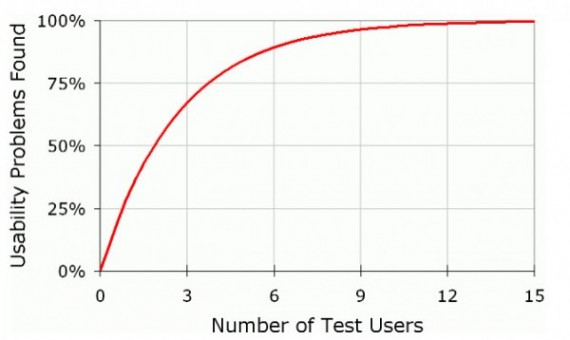
\includegraphics[scale=0.5]{Stichprobe.jpg}
	\caption{Stichprobengröße für Usability Tests}
	\label{fig2}
\end{figure}
\newpage
\section{Vorbereitung}
Für uns war es besonders wichtig zu sehen, ob Probanden die für sie unbekannte App, mühelos bedienen können und problemlos die vorgegebenen Ziele erreichen können.
Generelles Feedback, z.b. der Wunsch nach weiteren Funktionalitäten, war im Hinblick auf eine eventuelle Veröffentlichung der Applikation ebenfalls interessant für uns. \\
Unter diesen Gesichtspunkten haben wir folgendne Fragebogen (Abbilding 5.2) zusammengestellt, den die Probanden, nach Durchführung von festgelegten Aufgaben(Listing 5.1.), ausfüllen durften.\\
Um sicherzustellen, dass unsere Aufgaben und Befragung nicht zu viel Zeit in Anspruch nehmen, haben wir es vorher selbst durchgespielt und uns dabei bewusst Zeit gelassen.



\subsubsection*{Listing 5.1. Aufgabenliste}
\begin{itemize}
	\item 1.) Bearbeite dein Profil: Ändere den Namen und das Profilbild
	\item 2.) Plane zwischen 12 und 14 Uhr an der Cafeteria Essen zu gehen
	\item 3.) Trete einer Gruppe bei
	\item 4.) Schau dir das Profil eines Gruppenmitgliedes an
	\item 5.) Verlasse die Gruppe
	\item 6.) Erstelle eine eigene Gruppe
\end{itemize}
\newpage
\begin{figure}[H]
	\centering
  \includegraphics[scale=0.7]{Umfrage.pdf}
	\caption{Evaluationsbogen}
	\label{fig2}
\end{figure}
\newpage

\section{Durchführung}
Es wurden Personen auf dem KIT Campus, welche im Forum saßen, folgendermaßen angesprochen: \\
\ \\
\textit{Hallo, dürfen wir euch eine Frage stellen? Esst ihr regelmäßig in der Mensa?} \\ 
\ \\
Personen die diese Frage bejahten kamen als Probanden in Frage. \\
\ \\
\textit{Würdet ihr an einer kleinen Umfrage teilnehmen, es dauert nur 5 Minuten und als Dankeschön bekommt ihr ein paar Schoko Bons.}  \\ 
\ \\
Bei Zusage wurde eine Person aus der Personengruppe ausgewählt.\\
\ \\
\textit{Also, wir haben eine App entwickelt, mit der sich Leute anonym mit Fremden zum Essen gehen an der Mensa verabreden können und wir wollten uns etwas Feedback dazu einholen, deshalb darfst du die App jetzt kurz für uns testen. Du kriegst gleich ein Handy von uns, auf dem ist bereits ein User registriert und eingeloggt und dann musst du einfach diese sechs Aufgaben(zeigt Aufgabenliste) abarbeiten.} \\
\ \\
Während der Durchführung achteten wir auf die Zeit, schauten aufmerksam zu und notierten uns hinterher unsere Beobachtungen, die im Abschnitt Ergebnisse aufgeführt sind. \\
Nachdem die Aufgaben durchgeführt wurden erhielten die Probanden den Evaluatiosbogen.\\
\ \\
\textit{So, du hast jetzt während den Aufgaben alle Funktionalitäten der App kennen gelernt, jetzt musst du nur noch diesen Umfragebogen ausfüllen und dann bist du fertig.}

\newpage
\section{Ergebnisse}
Unser Test umfasste sieben Probanden, die alle auf oben beschriebene Weise am Campus angesprochen wurden.

\subsection*{Beobachtungen}
Die Probanden benötigten jeweils 5-7 Minuten für den gesamten Test, ab dem Zeitpunkt, ab dem sie das Handy und die Aufgabenliste bekamen. Hauptsächlich nahmen sie sich unterschiedlich viel Zeit für den Fragebogen.\\
\ \\
Zwei Probanden speicherten ihre Profiländerung nicht über den Speichern-Button sondern drückten stattdessen auf Zurück  um wieder in das Home Menü zu gelangen.
\ \\
Sechs von sieben Probanden haben nicht gemerkt, dass nicht nur drei sondern sechs Proflbilder zur Wahl standen.
\ \\
Beim Erstellen einer Gruppe ist die maximale Mitgliederzahl auf 1 einstellbar. 

\subsection*{Auswertung der Evaluationsbögen}
\ \\
\begin{tikzpicture}\begin{axis}[width=1.1\textwidth,height=0.6\textwidth,ybar,enlargelimits=0.1,symbolic x coords={Trifft nicht zu, Trifft eher nicht zu, Neutral, Trifft eher zu, Trifft voll zu}
,xtick={Trifft nicht zu, Trifft eher nicht zu, Neutral, Trifft eher zu, Trifft voll zu}, ylabel={Anzahl Antworten}]

\addplot[color=blue] coordinates{(Trifft nicht zu,0) (Trifft eher nicht zu,0) (Neutral,0) (Trifft eher zu,2) (Trifft voll zu,5)};
\addplot[color=red] coordinates{(Trifft nicht zu,1) (Trifft eher nicht zu,2) (Neutral,1) (Trifft eher zu,1) (Trifft voll zu,2)};
\addplot[color=green] coordinates{(Trifft nicht zu,0) (Trifft eher nicht zu,0) (Neutral,0) (Trifft eher zu,1) (Trifft voll zu,6)};

\end{axis} 
\end{tikzpicture}
\ \\
Legende: \ \\
Blau: Die App war intuitiv/leicht bedienbar. \\
Rot:  Ich würde diese App selber benutzen/weiterempfehlen. \\
Grün: Das Design hat mir gefallen.

\newpage
\subsection*{Antworten in den Freitextfeldern}

\subsubsection*{Wünscht du dir noch weitere Funktionen?}
Vier von sieben Probanden füllten dieses Feld aus: \\
\ \\
- Hashtags für die Gruppen zum Suchen \\
- Bewertungssystem für das Essen \\
- Aktualisieren des Essenplans, wenn etwas ausgegangen ist \\ 
- Bewerten von Essen und Personen \\
- Chat innerhalb der Gruppe

\subsubsection*{Was hat dir gefallen, was hat dir nicht gefallen?}
Zwei von sieben Probanden füllten dieses Feld aus: \\
\ \\
- Einfache Bedienbarkeit, Gute Funktionalität und vorrausschauendes Texting \\
- Hübsches Design \\
\ \\
\subsection*{Fazit}

TODO


\printglossaries
\end{document}